\documentclass[12pt,a4paper]{article}

\usepackage[utf8]{inputenc}
\usepackage[T1]{fontenc}
\usepackage{lmodern}
\usepackage[brazilian]{babel}
\usepackage[a4paper,margin=2.5cm]{geometry}
\usepackage{graphicx}
\usepackage{float}
\usepackage{booktabs}
\usepackage{xcolor}
\usepackage{caption}
\usepackage{hyperref}

\hypersetup{
    colorlinks=true,
    linkcolor=blue!50!black,
    urlcolor=blue!50!black,
    citecolor=blue!50!black,
    pdftitle={Integracao de Dados em Data Warehouse: ETL vs ELT aplicado ao CPGF},
}

% Identificador literal (sem interpretar _, #, etc.) para nomes de
% colunas, tabelas, arquivos e scripts.
\newcommand{\code}[1]{\texttt{\detokenize{#1}}}

\begin{document}

\begin{center}
\textbf{Universidade Federal de Pernambuco}

\textbf{Centro de Informática --- CIn}

\vspace{1cm}
{\LARGE Integração de Dados em Data Warehouse: ETL vs ELT aplicado ao CPGF}

\vspace{1cm}
% Logo do Centro de Informática (UFPE). Adicione o arquivo logo-cin.png
% nesta mesma pasta no Overleaf; se o arquivo não existir, esta linha não
% quebra a compilação.
\IfFileExists{logo-cin.png}{\includegraphics[width=3.5cm]{logo-cin.png}}{}

\vspace{1cm}
Relatório do Projeto de Integração\\
Banco de Dados --- 2026.2
\end{center}

\vspace{0.5cm}
\noindent
Flávio Araújo Filho --- fagpaf\\
João Pedro A. de Moraes --- jpam\\
Maria Cláudia Rocha --- mcsr

\vspace{0.8cm}

% =============================================================================
\section{Descrição da Base de Dados Unificada}
% =============================================================================

A base resultante é um \emph{Data Warehouse} em Esquema Estrela, em SQLite,
construído a partir de três anos (2023--2025) de dados do Cartão de
Pagamento do Governo Federal (CPGF), publicados pelo Portal da
Transparência. Ao todo são 438.771 transações (134.122 em 2023, 143.849 em
2024 e 160.800 em 2025), carregadas em uma tabela fato e cinco dimensões.

\begin{figure}[H]
    \centering
    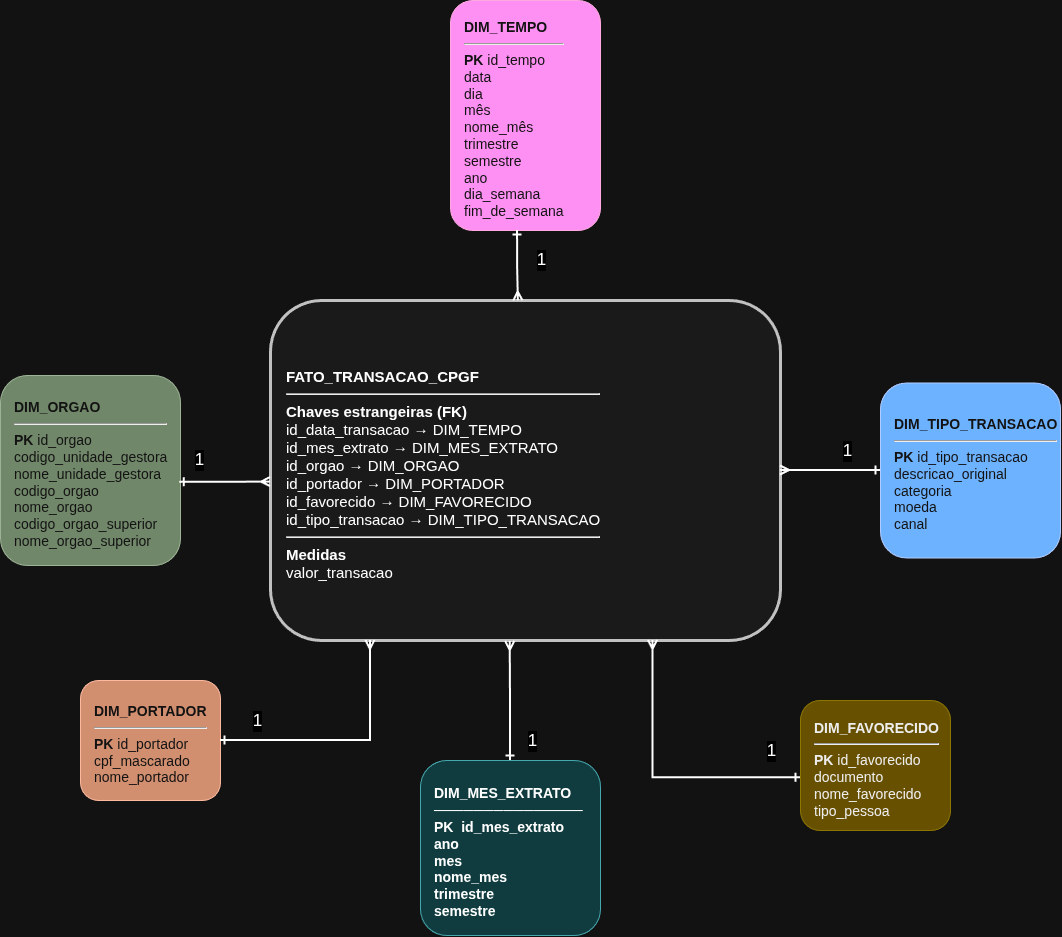
\includegraphics[width=0.85\textwidth]{../diagrams/diagrama-estrela.png}
    \caption{Esquema Estrela do data warehouse do CPGF.}
\end{figure}

A tabela \code{FATO_TRANSACAO_CPGF} tem grão de uma transação individual
(compra ou saque), com as medidas \code{valor_transacao} e
\code{quantidade_transacoes} (constante igual a 1, usada para contar
transações nas mesmas agregações de valor). As cinco dimensões, com a
quantidade de membros carregados, são:

\begin{itemize}
    \item \code{DIM_TEMPO} (1.462 linhas) --- dimensão de calendário com
    dois papéis: data da transação e mês do extrato;
    \item \code{DIM_ORGAO} (1.374) --- unidade gestora, órgão e órgão
    superior, desnormalizados em uma única tabela;
    \item \code{DIM_PORTADOR} (9.955) --- servidor responsável pelo cartão;
    \item \code{DIM_FAVORECIDO} (73.665) --- quem recebeu o pagamento,
    classificado em \code{PF}, \code{PJ} ou \code{Especial};
    \item \code{DIM_TIPO_TRANSACAO} (8) --- a descrição original da
    transação e os atributos derivados \code{categoria}, \code{moeda} e
    \code{canal}.
\end{itemize}

Cerca de 25\% das transações são sigilosas e não informam portador nem data
da compra; para não perder esses valores do total, \code{DIM_TEMPO} e
\code{DIM_PORTADOR} têm um membro especial \code{-1} que essas transações
usam no lugar de uma data ou portador reais.

Um detalhe relevante para quem for consultar o banco: \code{DIM_TIPO_TRANSACAO.moeda}
(valores \code{BRL}, \code{USD} ou ``Não Aplicável'') é uma classificação legada dos
pipelines e \textbf{não} é usada pelas análises de órgão e de favorecidos
(Seção~\ref{sec:analises}) --- o dicionário oficial do CPGF confirma que
\code{INT$} indica operação no exterior, mas não comprova que o valor
esteja em dólar, então essas duas análises passaram a agrupar pela descrição
original da transação (\code{R$/ATM}, \code{Exterior (INT$)} etc.) em vez
desse atributo. O racional completo está em
\code{docs/interpretacao-moedas-cpgf.md}.

O dicionário de dados completo (tipos, chaves e origem de cada coluna) está
em \code{docs/dicionario-de-dados.md}, e o racional de cada decisão de
modelagem em \code{docs/decisoes_modelagem.md}.

% =============================================================================
\section{Explicação Detalhada do Processo de Integração}
% =============================================================================

A integração seguiu quatro etapas, partindo sempre dos mesmos arquivos de
origem:

\begin{enumerate}
    \item \textbf{Coleta.} \code{scripts/extract_cpgf.py} baixa os pacotes
    mensais do Portal da Transparência e consolida cada ano em um CSV único
    (UTF-8, separado por \code{;}), além de gravar metadados (tamanho, hash
    SHA-256 e contagem de registros de cada arquivo).
    \item \textbf{Perfilamento.} \code{scripts/profile_cpgf.py} inspeciona
    os três CSVs antes de qualquer transformação, e identificou os
    problemas que guiaram a modelagem: sigilo, repetições exatas,
    defasagem entre data da compra e mês do extrato, e instabilidade das
    categorias de transação entre anos. Essa etapa só diagnostica; não
    altera os dados.
    \item \textbf{Modelagem.} A partir do diagnóstico, foram definidas as
    regras de transformação e o desenho do Esquema Estrela, detalhados na
    Seção~\ref{sec:transformacoes}.
    \item \textbf{Carga.} As mesmas regras foram implementadas duas vezes,
    em paralelo, por dois pipelines independentes --- ETL e ELT --- que
    geram dois bancos SQLite separados a partir dos mesmos CSVs
    (Seção~\ref{sec:comparativo}).
\end{enumerate}

A consolidação final é validada de forma independente dos próprios
pipelines: contagem de linhas, soma financeira em centavos e integridade
referencial são conferidas lendo diretamente os CSVs de origem, sem
reaproveitar nenhum número calculado pelos notebooks de carga. Na execução
de referência usada neste relatório, as 46 verificações realizadas
passaram para os dois bancos (ver Seção~\ref{sec:comparativo}).

% =============================================================================
\section{Justificativa da Escolha da Base de Dados}
% =============================================================================

O CPGF foi escolhido por três razões práticas. Primeiro, os dados são
públicos e podem ser baixados diretamente do Portal da Transparência, sem
necessidade de credenciais. Segundo, a série histórica permite comparar
três anos completos (2023--2025) com exatamente as mesmas 15 colunas, o que
viabiliza uma comparação justa entre os pipelines de ETL e ELT sobre o
mesmo volume de dados crescente ao longo do tempo. Terceiro, a base tem
complexidade suficiente para justificar um modelo dimensional de verdade:
uma hierarquia organizacional em três níveis, uma dimensão de tempo com
dois papéis distintos e uma fração grande e financeiramente relevante de
registros sob sigilo, que não poderia simplesmente ser descartada sem
distorcer qualquer soma de gastos.

% =============================================================================
\section{Descrição dos Processos de Transformação Aplicados}
\label{sec:transformacoes}
% =============================================================================

As regras abaixo foram aplicadas igualmente pelos dois pipelines (uma em
Python/pandas, a outra em SQL --- ver Seção~\ref{sec:comparativo}), e vieram
diretamente dos problemas identificados no perfilamento:

\begin{itemize}
    \item \textbf{Conversão de valores e datas.} Valores monetários no
    formato brasileiro (vírgula decimal) são convertidos para ponto, e
    datas no formato \code{dd/mm/aaaa} são padronizadas para o formato
    usado em \code{DIM_TEMPO}.
    \item \textbf{Tratamento de sigilo.} Transações sigilosas mantêm o
    valor e o mês do extrato, mas recebem o membro especial \code{-1} em
    \code{id_data_transacao} e \code{id_portador}, em vez de serem
    descartadas.
    \item \textbf{Classificação de favorecido.} \code{tipo_pessoa} é
    derivado do formato do documento após limpeza de pontuação: 14 dígitos
    viram \code{PJ}, 11 dígitos (ou a máscara de CPF da LGPD) viram
    \code{PF}, e marcadores administrativos da fonte (sigiloso, sem
    informação, não se aplica) viram uma categoria \code{Especial}
    separada.
    \item \textbf{Hierarquia organizacional.} Os três níveis administrativos
    do CSV (unidade gestora, órgão, órgão superior) são reunidos em uma
    única tabela \code{DIM_ORGAO}, deliberadamente desnormalizada.
    \item \textbf{Categoria residual de transação.} Como a lista de
    descrições de transação muda ligeiramente de um ano para outro, foi
    criada uma categoria \code{Outros} para as descrições que não se
    encaixam nos padrões já conhecidos de compra ou saque.
    \item \textbf{Repetições exatas não são removidas.} O perfilamento
    mostrou que, sobretudo sob sigilo, duas transações distintas podem ter
    exatamente os mesmos valores registrados; remover essas linhas poderia
    apagar transações legítimas, então nenhuma deduplicação automática é
    feita na carga.
\end{itemize}

% =============================================================================
\section{Comparativo entre ETL e ELT}
\label{sec:comparativo}
% =============================================================================

Os dois pipelines partem dos mesmos três CSVs anuais e aplicam as mesmas
regras da Seção~\ref{sec:transformacoes}; a diferença está em onde a
transformação acontece. No ETL (\code{notebooks/ETL.ipynb}), toda a limpeza
é feita em memória com \emph{pandas}, e só os dados já transformados chegam
ao banco (\code{cpgf_dw.sqlite}). No ELT (\code{notebooks/ELT.ipynb}), os
CSVs são carregados primeiro sem nenhuma alteração em tabelas
\code{raw_cpgf_*}, e a transformação é expressa inteiramente em SQL --- os
sete scripts de \code{scripts/sql/elt_transformations/} --- dentro do
próprio banco (\code{cpgf_elt.sqlite}).

A comparação quantitativa é feita pelo notebook
\code{notebooks/Benchmark_ETL_ELT.ipynb}, que mede tempo e pico de memória
de cada execução e valida os dois bancos de forma independente. Na
execução de referência (base completa, 438.771 transações, 3 repetições de
cada pipeline), as \textbf{46 verificações} de contagem, soma financeira,
integridade referencial, equivalência de atributos e tratamento de sigilo
passaram para os dois bancos --- ou seja, ETL e ELT chegam ao mesmo
resultado de negócio.

\begin{table}[H]
\centering
\caption{Comparativo de desempenho e características dos dois pipelines
(base completa, 438.771 transações, mediana de 3 repetições).}
\begin{tabular}{lrr}
\toprule
\textbf{Característica} & \textbf{ETL} & \textbf{ELT} \\
\midrule
Onde a transformação roda & Python / pandas (memória) & SQL dentro do SQLite \\
Tempo total, mediana & 14,23 s & 16,37 s \\
Pico de memória do kernel & 678 MB & 80 MB \\
Tamanho do banco gerado & 54,91 MB & 302,96 MB \\
Tabelas no banco & 6 & 10 \\
Guarda o dado bruto no banco & Não & Sim \\
Linhas de código Python no notebook & 350 & 263 \\
Linhas de SQL de transformação & 0 & 235 \\
Usa \emph{pandas} & Sim & Não \\
\bottomrule
\end{tabular}
\end{table}

A diferença de tempo entre as duas abordagens é pequena nesta execução; a
diferença marcante está na memória --- o pico do ETL é cerca de 8,5 vezes
maior que o do ELT, porque todo o conjunto de dados passa pela memória do
kernel Python antes de chegar ao banco. Em compensação, o banco do ELT é
quase 6 vezes maior, porque mantém as tabelas \code{raw_cpgf_*} com os
dados brutos além do Esquema Estrela já transformado, enquanto o ETL não
guarda o dado bruto em lugar nenhum. O ETL concentra toda a lógica em um
único notebook de 350 linhas, mais simples de acompanhar e depurar; o ELT
distribui a mesma lógica entre um notebook menor e sete scripts SQL
específicos, o que deixa cada regra de transformação isolada, mas espalha
a lógica por mais arquivos.

Para um projeto como este, com uma carga em lote de um volume de dados
conhecido (e não uma ingestão contínua), as duas abordagens são viáveis: o
ETL é preferível quando se quer depurar a transformação em Python e manter
tudo em um lugar só; o ELT é preferível quando se quer auditar o dado bruto
depois da carga ou manter as regras de negócio expressas em SQL dentro do
próprio banco. Tempo e memória medidos variam conforme a máquina e a carga
do sistema no momento da execução, então esses números devem ser lidos como
uma comparação relativa entre as duas abordagens, não como uma medição
absoluta e definitiva.

% =============================================================================
\section{Apresentação de Três Análises e Insights}
\label{sec:analises}
% =============================================================================

Três análises foram construídas sobre o data warehouse resultante, cada uma
com uma consulta SQL, um script Python que gera o gráfico correspondente e
um documento descrevendo as decisões metodológicas.

\subsection{Evolução temporal e sazonalidade}

O eixo de tempo usado é o mês do extrato (\code{id_mes_extrato}), e não a
data da compra: cerca de 25\% das transações são sigilosas e não informam a
data da compra, mas todas informam o mês do extrato, então esse eixo
preserva 100\% do valor analisado.

\begin{table}[H]
\centering
\caption{Evolução anual do CPGF, 2023--2025.}
\begin{tabular}{lrrr}
\toprule
\textbf{Ano} & \textbf{Transações} & \textbf{Valor total (R\$)} & \textbf{Ticket médio (R\$)} \\
\midrule
2023 & 134.122 & 90.717.210,79 & 676 \\
2024 & 143.849 & 111.802.599,28 & 777 \\
2025 & 160.800 & 122.254.704,02 & 760 \\
\bottomrule
\end{tabular}
\end{table}

\begin{figure}[H]
    \centering
    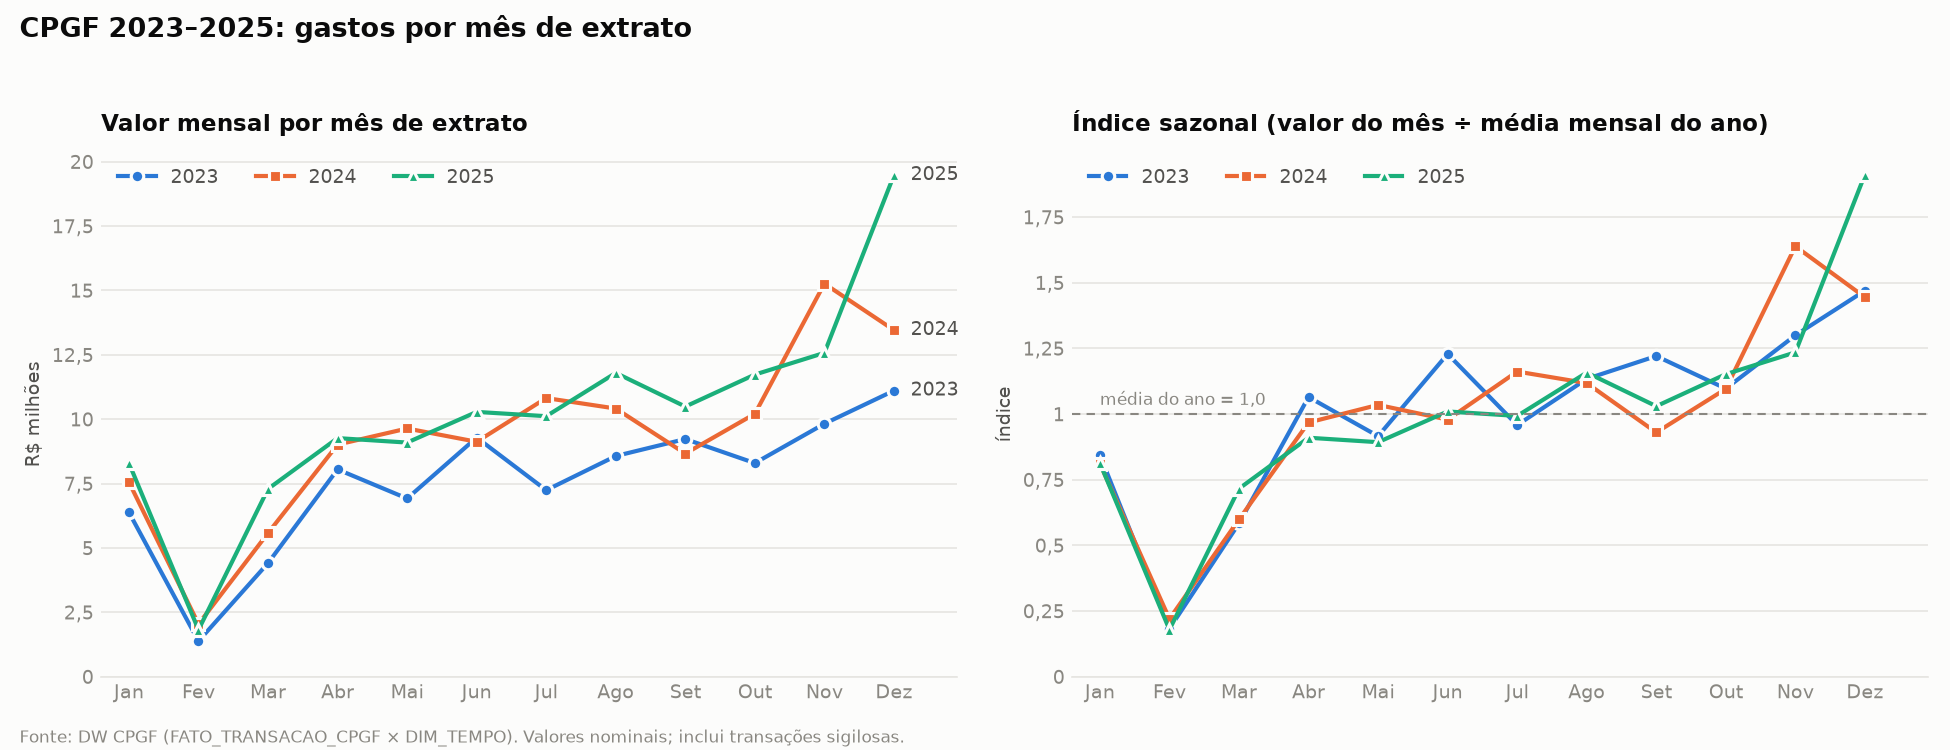
\includegraphics[width=0.9\textwidth]{../analises/01_analise/evolucao-temporal.png}
    \caption{Valor mensal e índice sazonal por ano.}
\end{figure}

O crescimento desacelera: +23,2\% em valor de 2023 para 2024 (puxado
principalmente pelo ticket médio, que sobe 15\%), e +9,3\% de 2024 para
2025 (desta vez puxado mais pela quantidade de transações, que cresce
11,8\%, enquanto o ticket médio recua). Nos três anos, novembro e dezembro
concentram entre 23\% e 26\% do valor anual, e fevereiro é sistematicamente
o mês mais fraco (índice sazonal entre 0,18 e 0,22 da média do ano) --- a
causa dessa queda não foi investigada nesta análise.

\subsection{Gastos por órgão e proporção de transações sigilosas}

A segunda análise agrupa os gastos pelo órgão superior e investiga, por
grupo de operação (\code{R$/ATM}, \code{Exterior (INT$)} e sigilosas),
quais órgãos concentram os maiores valores e qual fração de suas
transações é classificada como sigilosa. O ranking em \code{R$/ATM} não
representa o gasto total do órgão, só o recorte de compras e saques nessa
moeda.

\begin{figure}[H]
    \centering
    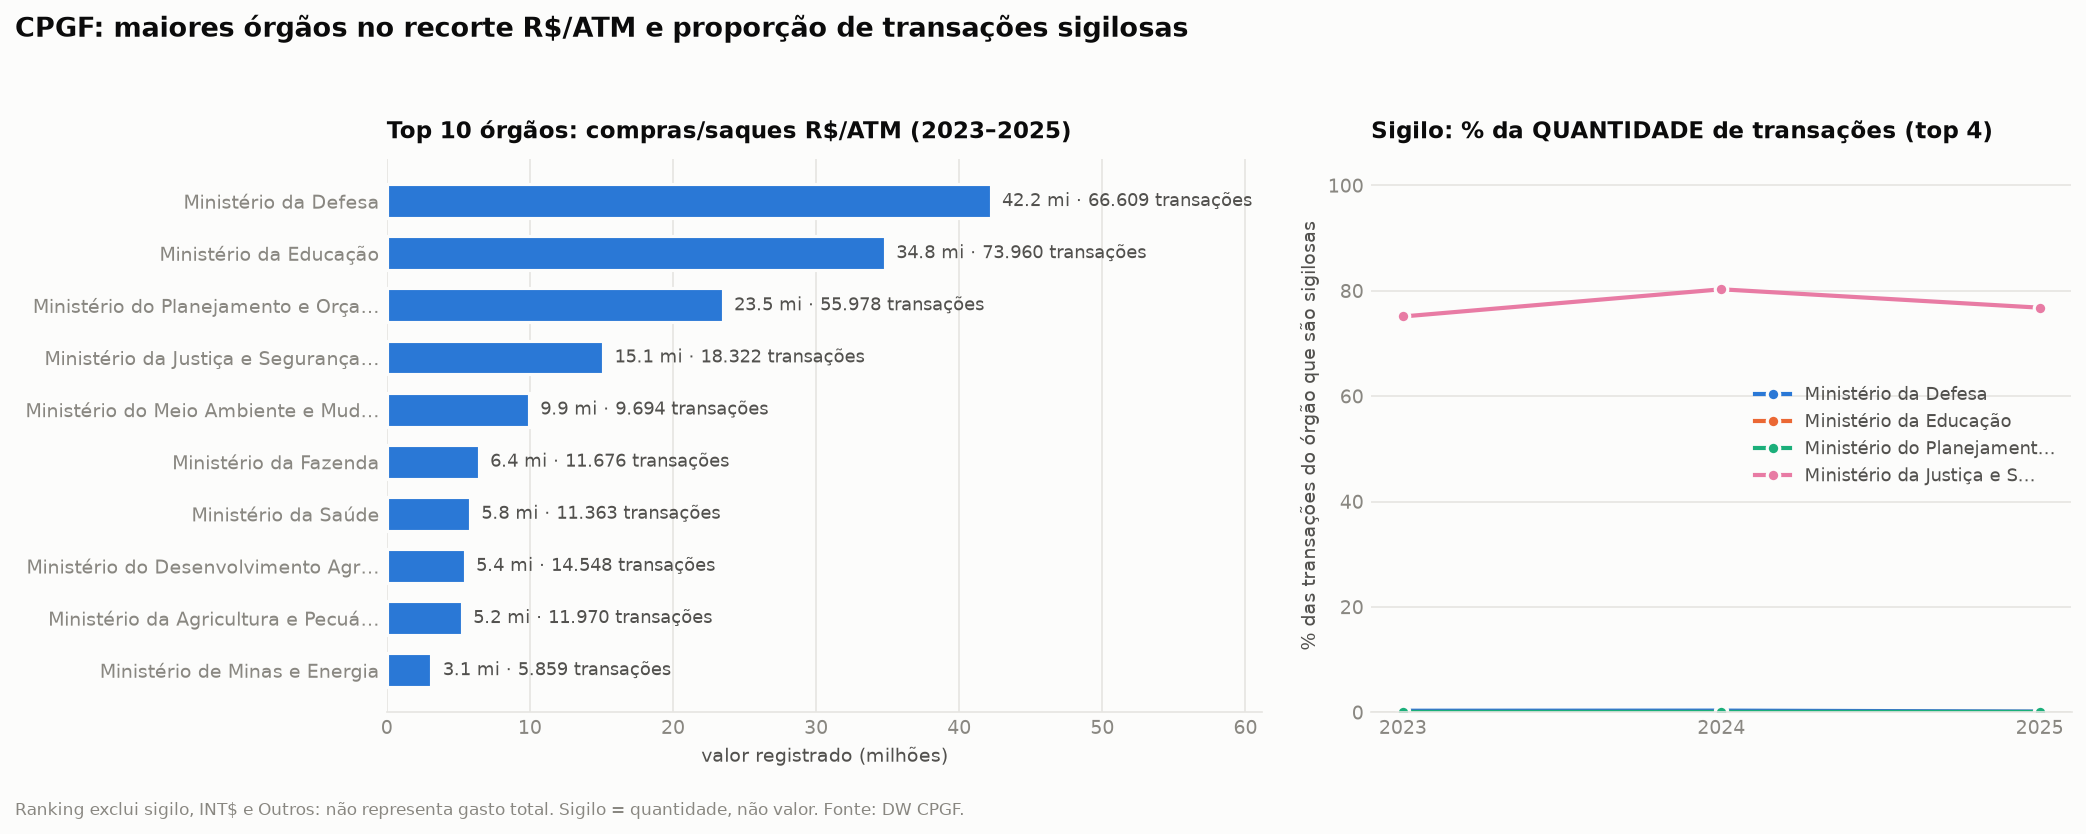
\includegraphics[width=0.95\textwidth]{../analises/02_analise/analise_gastos_por_orgao.png}
    \caption{Maiores órgãos superiores em R\$/ATM (2023--2025) e evolução
    anual da parcela sigilosa.}
\end{figure}

Os cinco maiores órgãos superiores no recorte \code{R$/ATM} são o
Ministério da Defesa (R\$~42,2 milhões, 66.609 transações), o Ministério da
Educação (R\$~34,8 milhões), o Ministério do Planejamento e Orçamento
(R\$~23,5 milhões), o Ministério da Justiça e Segurança Pública
(R\$~15,1 milhões) e o Ministério do Meio Ambiente e Mudança do Clima
(R\$~9,9 milhões). O padrão de sigilo não acompanha o volume financeiro:
Defesa, Educação e Planejamento têm proporção de transações sigilosas
praticamente nula nos três anos, enquanto o Ministério da Justiça e
Segurança Pública se destaca com entre 75\% e 80\% de suas transações
classificadas como sigilosas em todos os anos observados.

\subsection{Tipos de transação e concentração em favorecidos}

A terceira análise compara compras com saques e investiga a concentração de
valores entre os favorecidos (\code{DIM_FAVORECIDO}).

\begin{figure}[H]
    \centering
    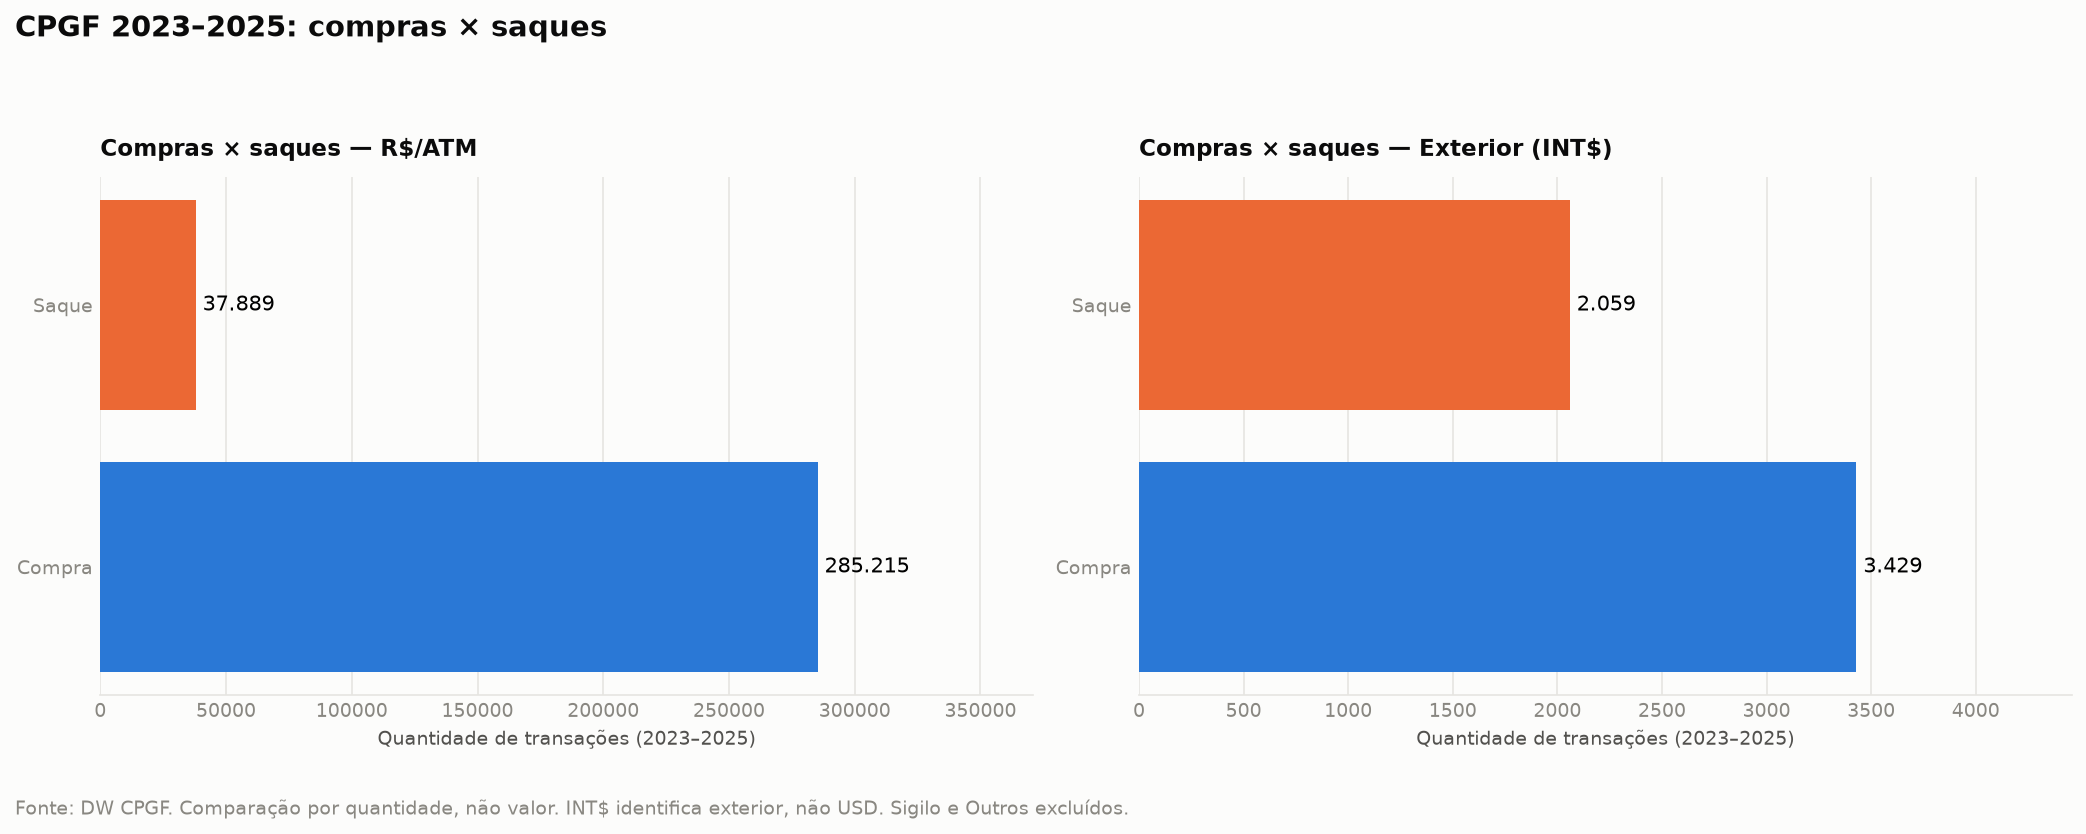
\includegraphics[width=0.95\textwidth]{../analises/03_analise/compras_saques.png}
    \caption{Compras e saques por grupo de operação, em quantidade.}
\end{figure}

\begin{figure}[H]
    \centering
    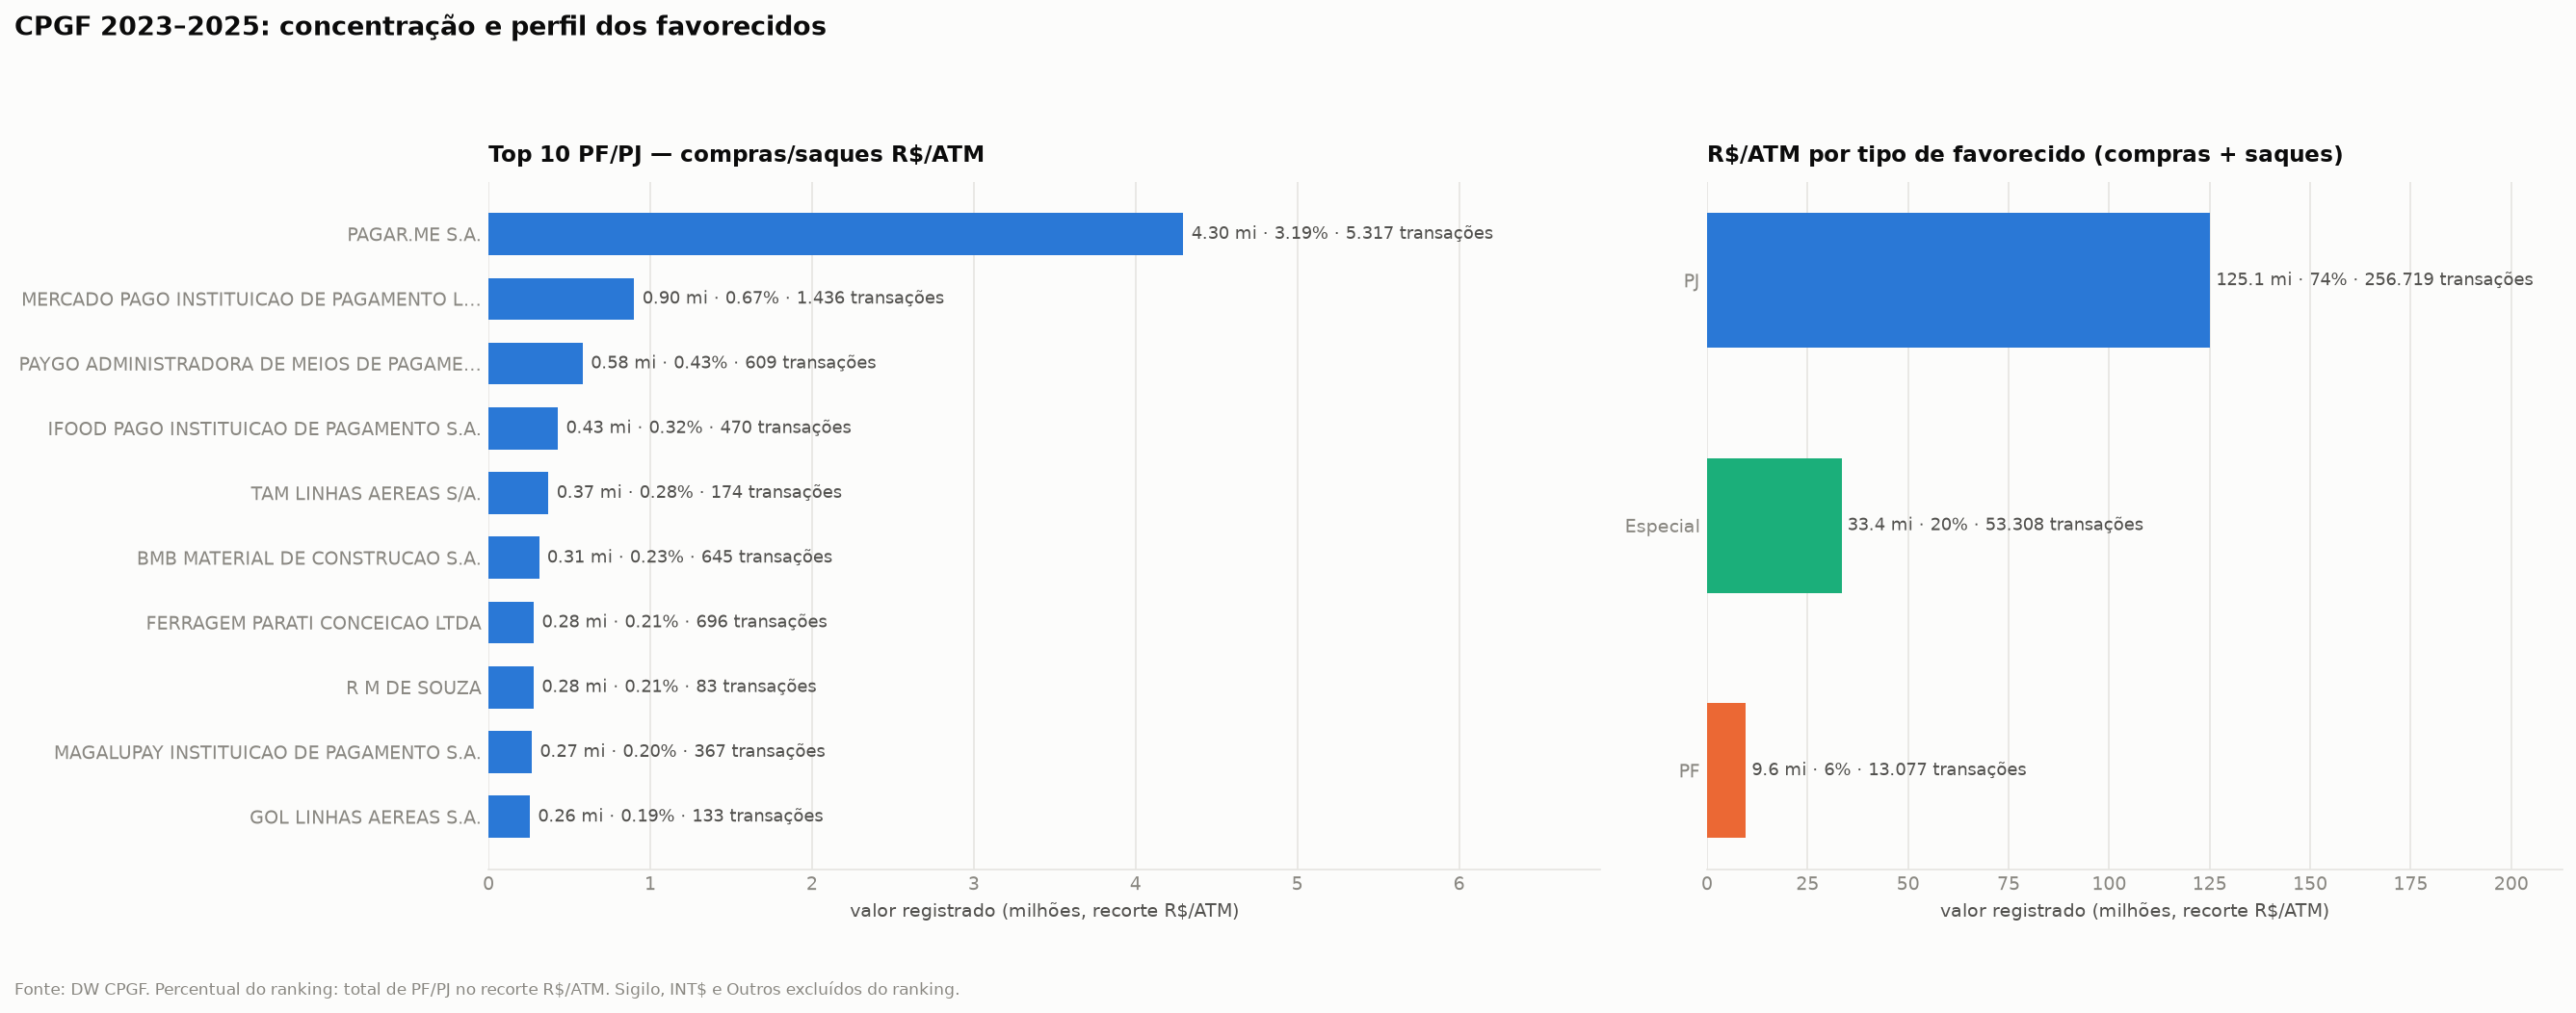
\includegraphics[width=0.95\textwidth]{../analises/03_analise/concentracao_favorecidos.png}
    \caption{Maiores favorecidos identificados em R\$/ATM e distribuição por
    tipo de favorecido.}
\end{figure}

Em quantidade, compras superam saques com folga nas duas moedas (285.215
compras contra 37.889 saques em \code{R$/ATM}; 3.429 contra 2.059 no
recorte \code{Exterior (INT$)}). O maior favorecido identificado (pessoa
física ou jurídica) é a \code{PAGAR.ME S.A.} (PJ), com 5.317 transações e
R\$~4.295.670,12, equivalente a 3,19\% do total considerado no ranking. Um
resultado notado explicitamente na análise: as 5.488 transações do recorte
\code{Exterior (INT$)} são \emph{todas} associadas a favorecidos do tipo
\code{Especial} --- não há, nos dados disponíveis, nenhum favorecido
\code{PF} ou \code{PJ} identificado nesse recorte.

% =============================================================================
\section{Reflexão sobre o Aprendizado}
% =============================================================================

A maior dificuldade técnica do projeto não foi escrever as consultas, mas
decidir o que fazer com os registros sigilosos: cerca de um quarto da base
não informa data da compra nem portador, e simplesmente descartar essas
linhas teria subestimado os gastos reais de órgãos inteiros (como ficou
claro na análise da Seção~\ref{sec:analises}, em que um único órgão
concentra a maior parte do sigilo). Resolver isso exigiu uma decisão de
modelagem explícita --- os membros especiais \code{-1} --- em vez de uma
solução genérica de limpeza de dados.

Implementar as mesmas regras de negócio duas vezes, em paradigmas
diferentes (pandas em memória e SQL dentro do banco), também mostrou na
prática uma diferença que não aparece só em documentação: o ETL concentra
tudo em um único notebook, mais fácil de acompanhar passo a passo, enquanto
o ELT obriga a pensar em cada transformação como uma consulta
independente, o que separa melhor as responsabilidades mas exige mais
disciplina para manter as duas camadas (bruta e transformada) consistentes.
A comparação de desempenho reforçou esse ponto: a diferença de tempo entre
as duas abordagens foi pequena, mas a diferença de memória foi grande o
suficiente para mudar a recomendação dependendo do ambiente de execução
disponível --- em uma máquina com pouca memória, o ELT seria a escolha mais
segura, mesmo gerando um banco maior.

% =============================================================================
\section*{Referências}
% =============================================================================

\begin{itemize}
    \item Portal da Transparência do Governo Federal --- Cartão de
    Pagamento do Governo Federal (CPGF):
    \url{https://portaldatransparencia.gov.br/download-de-dados/cpgf}
\end{itemize}

\end{document}
